\chapter{RF-Score-v4: impact of pose generation error}

\section{Abstract}

This was a collaborative project with Pedro J. Ballester from Cancer Research Center of Marseille, Marseille, France. It was published in the \textit{Proceedings of the 11th International Meeting on Computational Intelligence Methods for Bioinformatics and Biostatistics (CIBB)} on 26 June 2014 \citep{1434}.

\section{Introduction}

To avoid confounding factors introduced by pose generation, these studies on scoring accuracy are carried out on data consisting of large sets of X-ray structures of protein-ligand complexes. However, scoring of the docked poses of a molecule is required in those cases where the experimentally-determined pose is not available.

In this paper, we study the impact of pose generation error on classical and machine-learning scoring functions. Furthermore, we investigate which of these scoring functions is more suitable for predicting the near-native pose (i.e. the most similar docked pose to the co-crystallised pose). The numerical experiments will be performed with AutoDock Vina [7], as the classical scoring function, and RF-Score [2] as the machine-learning scoring function. Investigating the generalisation of these results to other non-parametric machine learning techniques previously applied to this problem, such as SVR in [8], is out of the scope of this study, although expected to yield similar outcomes.

\section{Methods}

Four models, same as the previous chapter, except: 1) 11 features, Vina math expression, 2) MLR::Vina w6 range.

\subsection{Experimental design}

Each of the 1300 co-crystallised ligands is redocked into the binding site of its target protein using Vina. For each molecule, this results in a maximum number of nine docked poses. The Root-Mean Square Deviation (RMSD) quantifies how different the 3D geometry of the redocked pose is from the corresponding co-crystallised pose of the same ligand molecule (i.e. the pose generation error). Because we aim at investigating the impact of pose generation error on the prediction of binding affinity, a second test set is defined where each of the 195 complexes has its ligand re-docked and its binding affinity predicted by scoring functions trained on the 1105 crystal structures. As a baseline, these scoring functions are also tested on the co-crystallised ligands of the same 195 complexes.

\section{Results}

It is noteworthy that, in redocked poses, Vina achieved a relatively small pose generation error in the test set (52\% of the ligands had a docked pose with RMSD < 2\AA). In terms of scoring accuracy, performance is measured as the Root Mean Square Error (RMSE), Pearson’s correlation coefficient (Rp) and the Spearman’s rank-correlation coefficient (Rs) between measured and predicted binding affinity. Figure 1 shows the performance of the four scoring functions when tested on co-crystallised poses and redocked poses of the same complexes. These results show that pose generation error introduces a small degradation in the ability to rank-order complexes according to predicted binding affinity in all scoring functions (see Rs plot). In terms of scoring power (Rp and RMSE), RF-based scoring functions performs slightly worse on docked poses (models 3-4). In contrast, those assuming a functional form do slightly better on docked poses (models 1-2). The latter is likely to be due to the fact that docked poses are by construction optima of the objective function spanned by the Vina score, which may favour prediction of docked poses over unoptimised co-crystallised ligands. On the other hand, it is remarkable that the best scoring function, RF::VinaElem, achieves the highest performance in the literature on this test set in the more common application of re-scoring docked poses. Importantly, since models 1 and 3 use the same features and are trained on the same data, RF::Vina performs much better at predicting binding affinity than the widely-used Vina while having the same applicability domain.

\begin{figure}
\centering
\subfloat{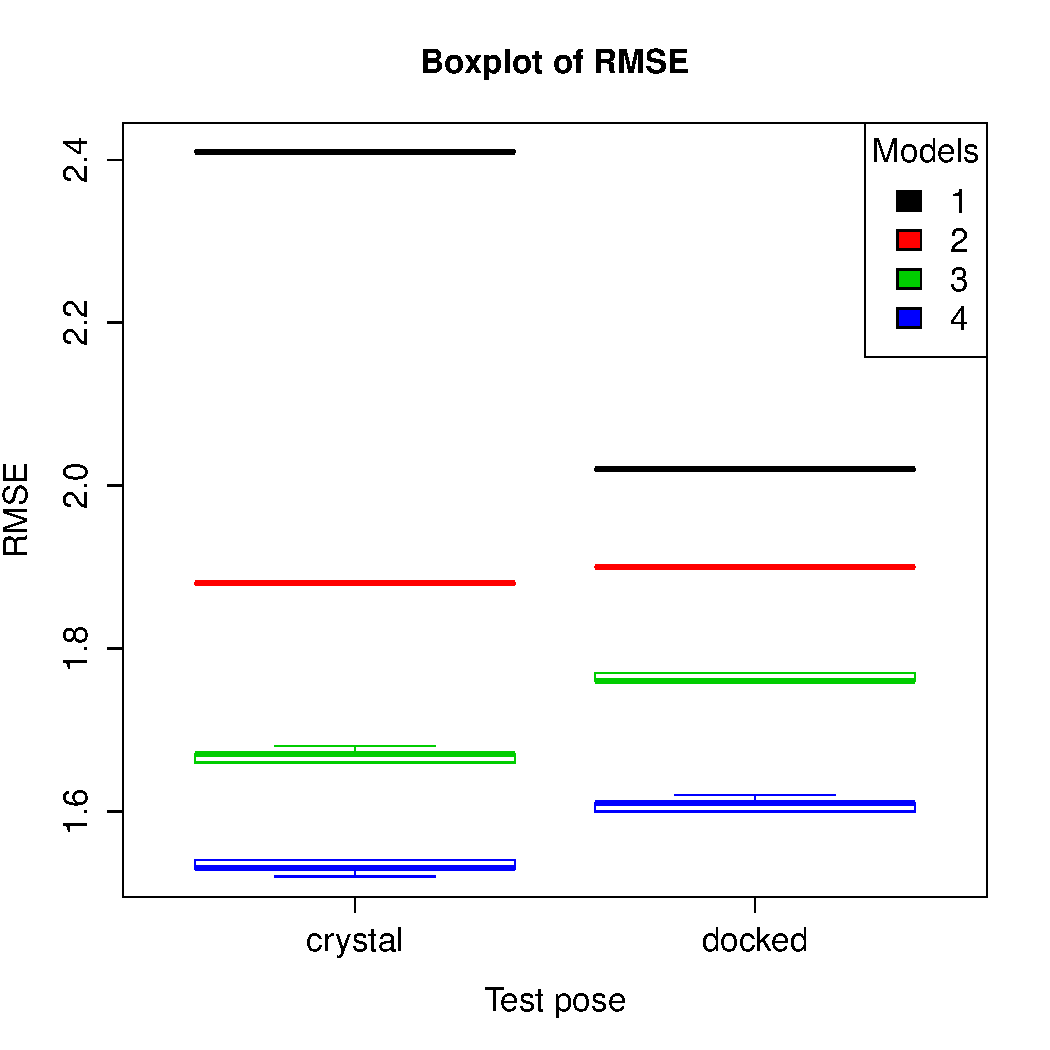
\includegraphics[width=0.24\linewidth]{../rfscore4/set-1-pdbbind-2007-trn-1-rmse-boxplot.pdf}}
\subfloat{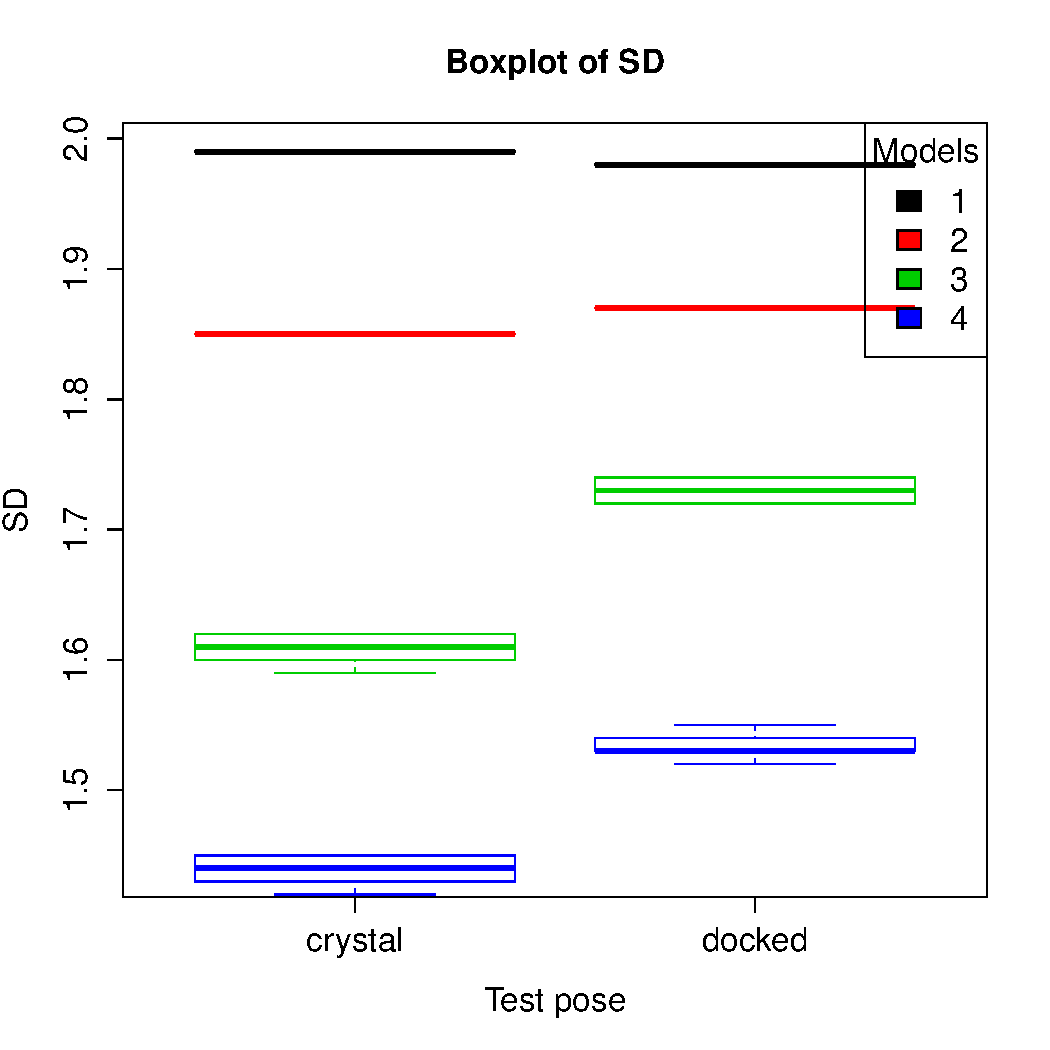
\includegraphics[width=0.24\linewidth]{../rfscore4/set-1-pdbbind-2007-trn-1-sdev-boxplot.pdf}}
\subfloat{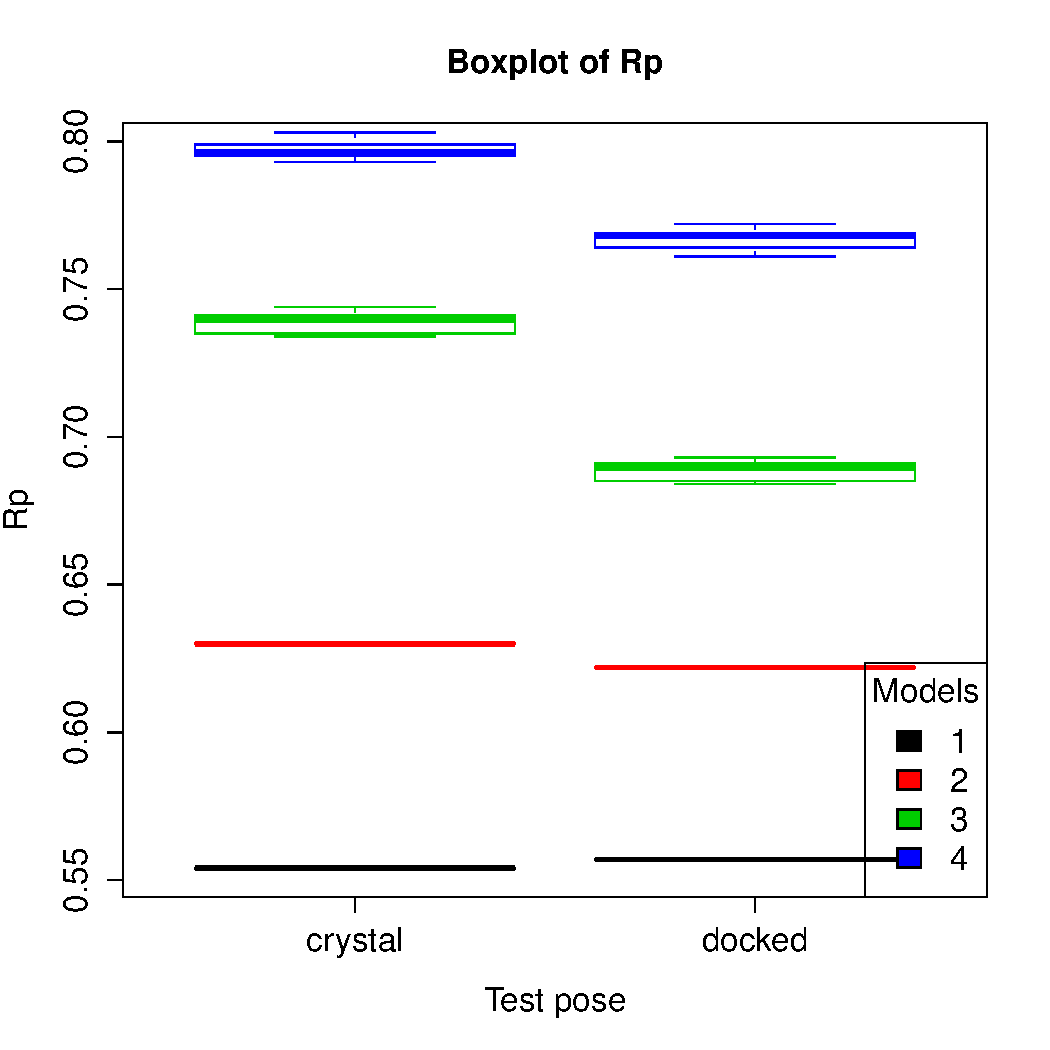
\includegraphics[width=0.24\linewidth]{../rfscore4/set-1-pdbbind-2007-trn-1-pcor-boxplot.pdf}}
\subfloat{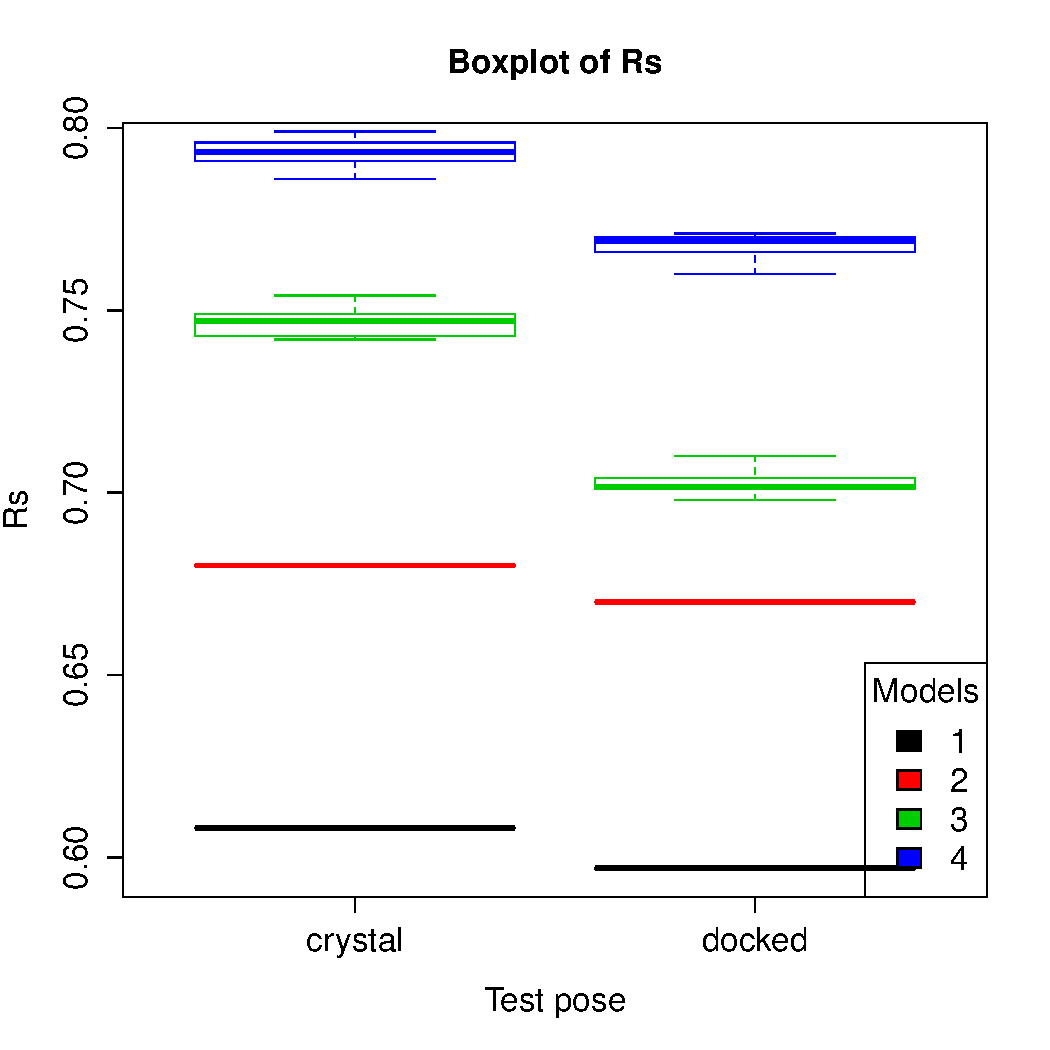
\includegraphics[width=0.24\linewidth]{../rfscore4/set-1-pdbbind-2007-trn-1-scor-boxplot.pdf}}
\caption{Performance of each scoring function on the PDBbind v2007 core set test set with co-crystallised ligands (left of each plot) and the set of complexes with the re-docked ligand with the lowest Vina score instead (right).}
\label{rfscore4:set-1-pdbbind-2007-trn-1}
\end{figure}

\begin{figure}
\centering
\subfloat{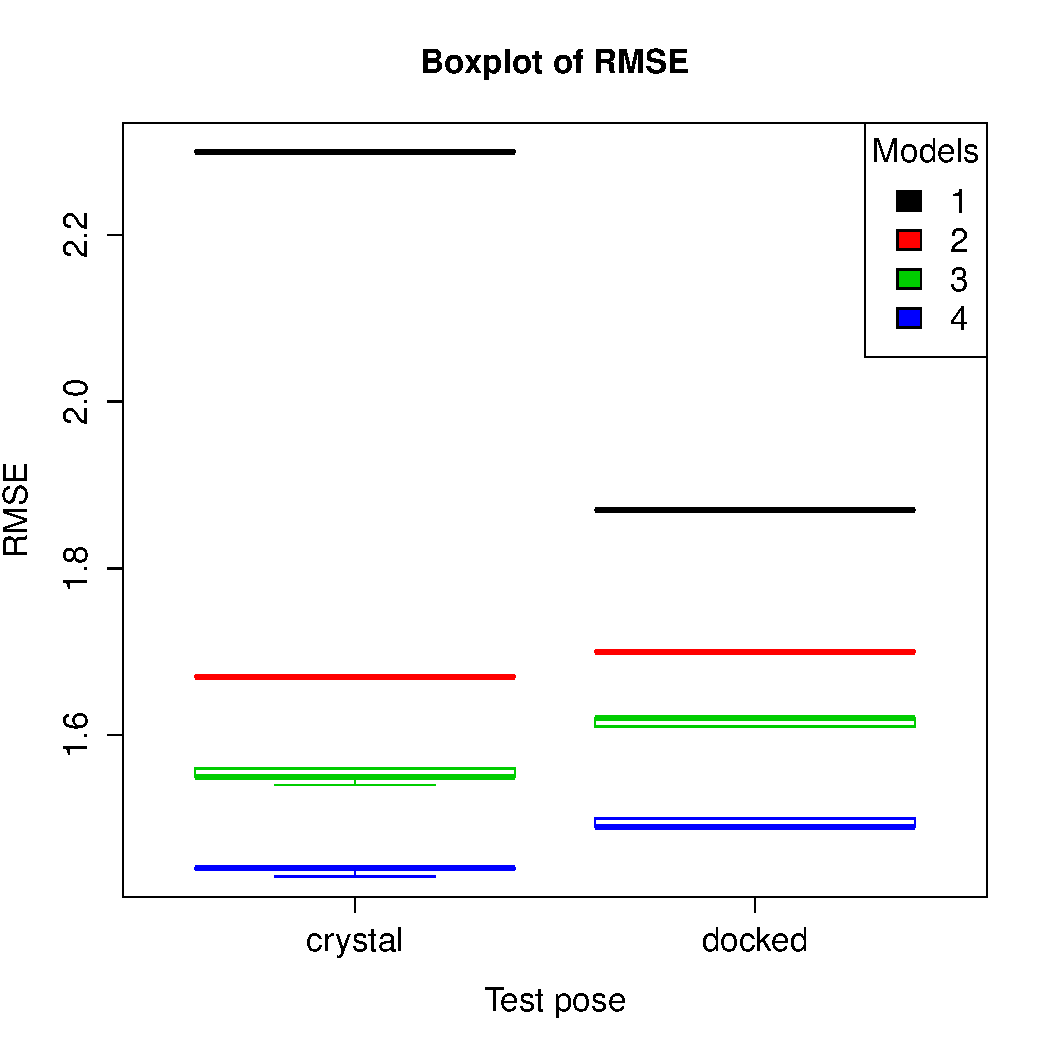
\includegraphics[width=0.24\linewidth]{../rfscore4/set-2-pdbbind-2012-trn-1-rmse-boxplot.pdf}}
\subfloat{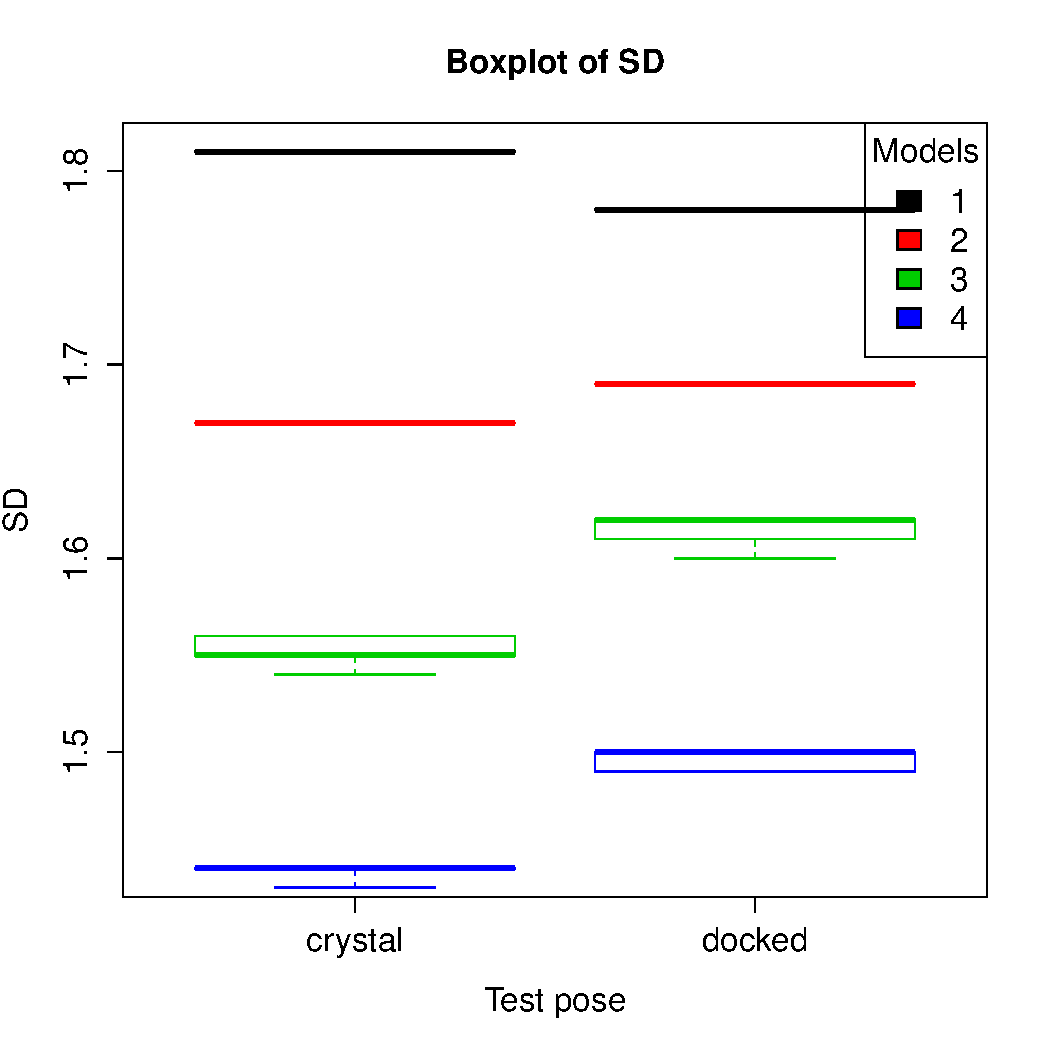
\includegraphics[width=0.24\linewidth]{../rfscore4/set-2-pdbbind-2012-trn-1-sdev-boxplot.pdf}}
\subfloat{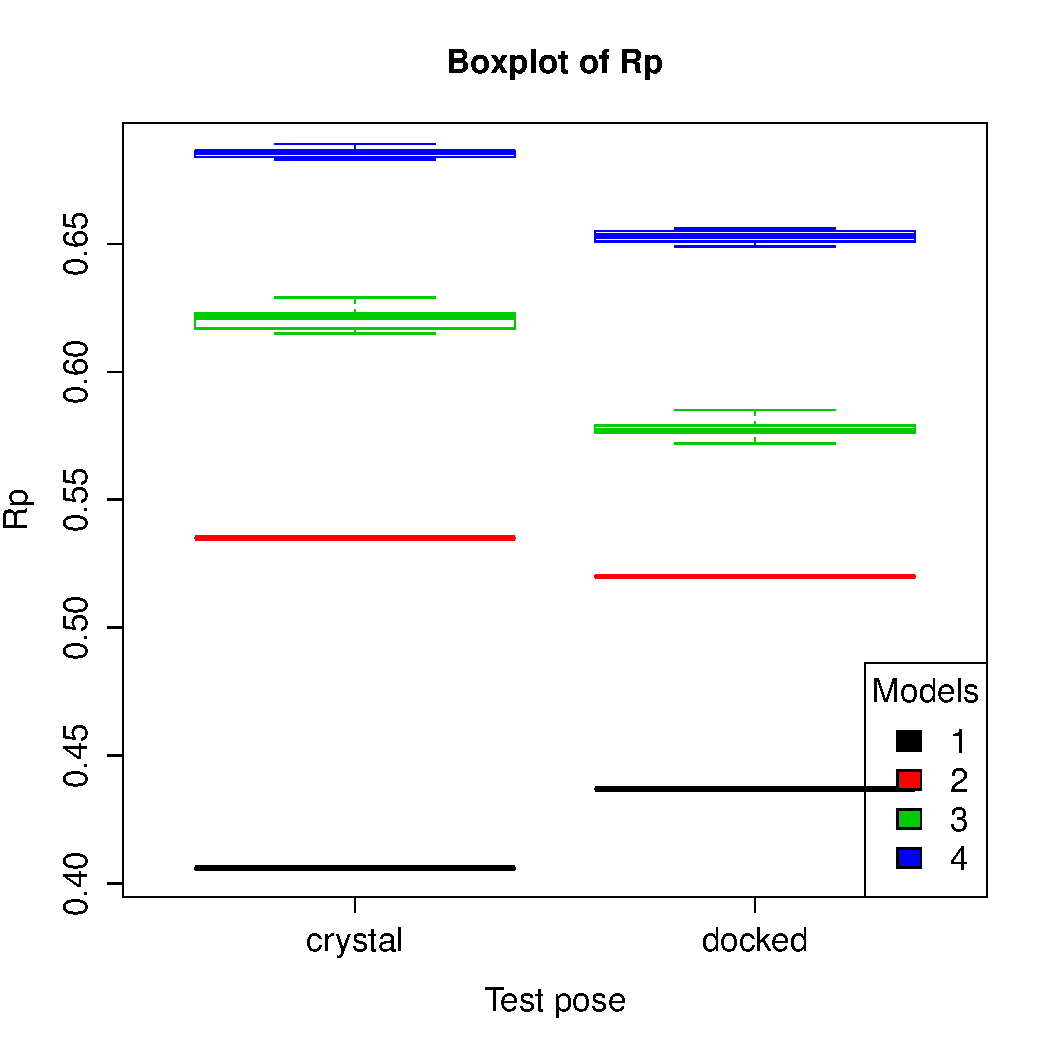
\includegraphics[width=0.24\linewidth]{../rfscore4/set-2-pdbbind-2012-trn-1-pcor-boxplot.pdf}}
\subfloat{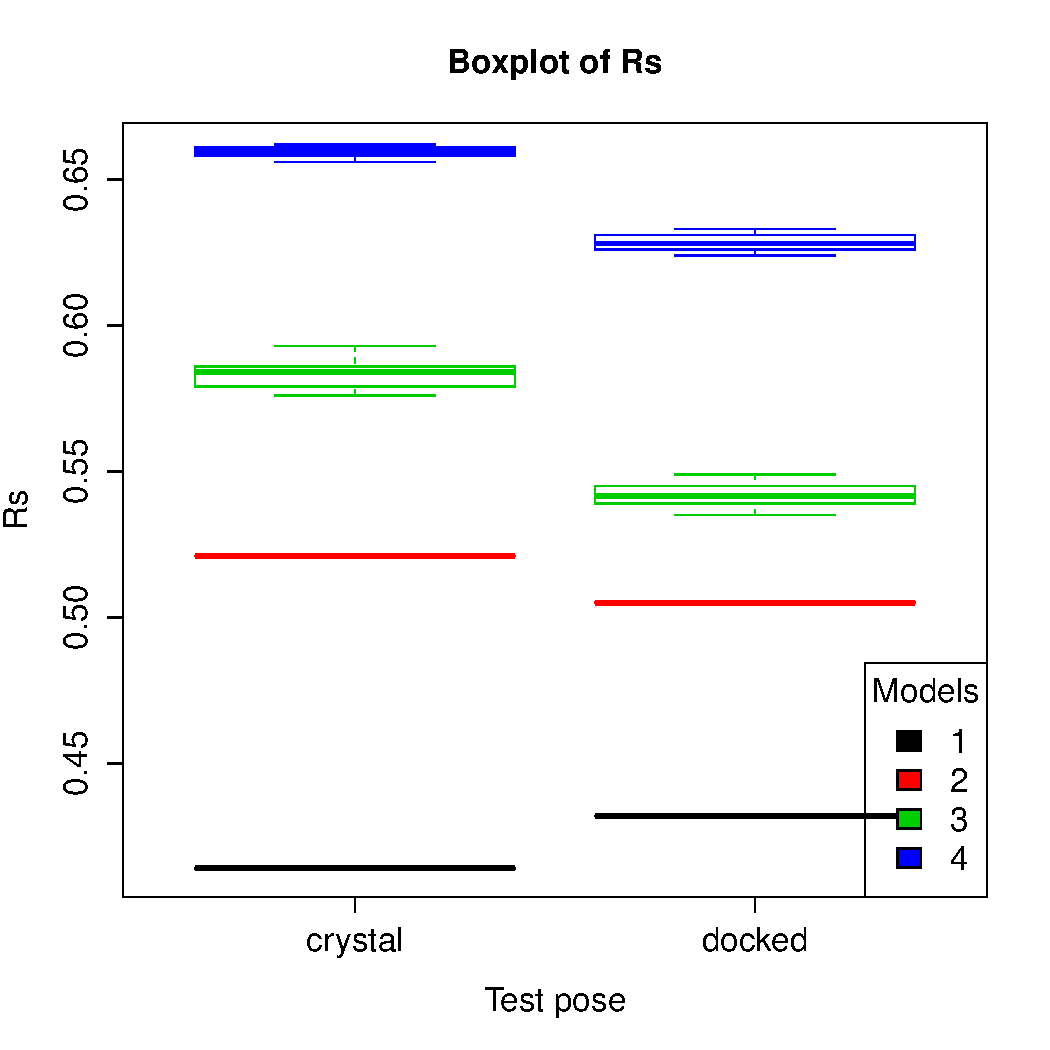
\includegraphics[width=0.24\linewidth]{../rfscore4/set-2-pdbbind-2012-trn-1-scor-boxplot.pdf}}
\caption{Performance of each scoring function on the PDBbind blind benchmark test set with co-crystallised ligands (left of each plot) and the set of complexes with the re-docked ligand with the lowest Vina score instead (right).}
\label{rfscore4:set-2-pdbbind-2012-trn-1}
\end{figure}

Next, we assess the ability of each scoring function to predict the near-native pose of a molecule as bound to a target (see Table 1). Interestingly, results show that the least accurate predictor of binding strength in this study (Vina) is the best at predicting which docked pose is geometrically the closest to the co-crystallised pose. In contrast, the presented machine-learning scoring functions, while excelling at binding affinity prediction, perform much worse than Vina at native pose prediction. This suggests that these two tasks, binding affinity prediction and native pose prediction, cannot be optimally covered by a single scoring function.

\section{Conclusions}

This study has demonstrated that errors in pose generation generally introduce a small error in the accuracy of scoring. Furthermore, RF::VinaElem obtained the highest performance on this test set in the common scenario where one has to predict the binding affinity of docked poses instead of those for co-crystallised poses (usually because a crystal structure of the ligand is not available). Nevertheless, we observed that the presented machine-learning scoring functions do not perform well at predicting the near native pose of a ligand. In the future, we intend to investigate scoring functions tailored to this related problem.

\section{Future works}

Repeat experiments with idock instead of Vina.

\chapterend
